
%   Template - Institute of Control Systems, TUHH

%#############################################################################
%     R E A D      M E     F I R S T  !
%#############################################################################
% For setting up a latex enviroment, please follow: https://www.latexbuch.de/latex-windows-installieren/
% In Texmaker you can setup fast compile with these arguments: lualatex -interaction=nonstopmode %.tex|biber %|lualatex -interaction=nonstopmode %.tex|"C:/Program Files/Adobe/Reader 11.0/Reader/AcroRd32.exe" %.pdf
% Possible compilation processes:
% Luatex -> biber -> Luatex 
% For texstudio: lualatex.exe -synctex=1 -interaction=nonstopmode --enable-write18 -interaction=nonstopmode %.tex or pdflatex.exe -synctex=1 -interaction=nonstopmode -shell-escape --enable-write18 -interaction=nonstopmode %.tex
% enables the compiler to use tikz externalize as well
% Toolchain is than: PDFLatex: txs:///pdflatex | txs:///biber | txs:///pdflatex | txs:///view-pdf-internal --embedded
%					  LuaLatex: txs:///lualatex | txs:///biber | txs:///lualatex | txs:///view-pdf-internal --embedded
% VS-Code + LatexWorkshop: Config-File in header/VS_Settings.json
%#############################################################################

%%################ Language settings #########################################
\def\isenglish{true}	% change to false for German language

%%################ DRAFT settings ############################################
\def\isDraft{true}		% Change to false for final project description

 %%################ Document settings #########################################
\def\curdir{}
%%%%%%%%%%%%%%%% Document settings %%%%%%%%%%%%%%%%%%%%
%\NeedsTeXFormat{LaTeX2e}
\documentclass[a4paper,12pt]{article}
\usepackage{ifluatex}\usepackage{microtype}
\ifluatex
	\usepackage{fontspec}
\else
	\usepackage[utf8]{inputenc}
\fi

\usepackage{graphicx}                %% special graphics
\usepackage{color}                   %% allow colour
\usepackage{xcolor}
\usepackage{latexsym}                %% symbols package
\usepackage{amsmath}                 %% special mathematical functions
\usepackage{theorem}
\usepackage{amsfonts}
\usepackage{ifthen}
\usepackage[style=ieee,backend=biber]{biblatex} %% bibliography
\usepackage{csquotes}
\usepackage{multirow}                %% multirow tables
\usepackage{booktabs}                %% make tables look nice
\usepackage{enumerate}
\usepackage{lmodern}
\usepackage{subcaption}
\usepackage{tikz}

\ifthenelse{\equal{\isDraft}{true}}
{
  \usepackage[firstpageonly, color=red, text=DRAFT\\Version, scale=0.25, vanchor=t, angle=30, pos={14cm,5cm}]{draftwatermark}
}
{}

\usetikzlibrary{%
  arrows,%
  arrows.meta,
  shapes.misc,% wg. rounded rectangle
  shapes.arrows,
  shapes.misc,
  calc,
  plotmarks,
  chains,%
  matrix,%
  positioning,% wg. " of "
  scopes,%
  decorations.pathmorphing,% /pgf/decoration/random steps | erste Graphik
  decorations.markings,
  shadows%
}
\usetikzlibrary{external}
\tikzexternalize[prefix=figures/externalize/] % activate!
\usepackage{pgfplots}
\pgfplotsset{compat=newest}

\newlength{\figw}
\setlength{\figw}{0.8\textwidth}
\newlength{\figh}
\setlength{\figh}{0.4\textwidth}

\newcommand{\tikzfig}[2]{
  \tikzsetnextfilename{#2}%
  \scalebox{#1}{
    \input{"figures/#2.tex"}}
}

% Listings
\usepackage{listings} \lstset{numbers=left, numberstyle=\tiny, numbersep=5pt, frame=single} 
%\lstset{basicstyle=\ttfamily}
\lstset{language=matlab,emph={lsim, ones, feedback},emphstyle=\textbf, identifierstyle=\ttfamily}

%%############### Choose LANGUAGE
\ifthenelse{\equal{\isenglish}{true}}{
 %%% English
	\usepackage[german, ngerman, english]{babel}
	\selectlanguage{english}
    \def\bibnamep{References}%
    \def\bibnamem{References}%
}{
%%% German
	\usepackage[english, german, ngerman]{babel}
	\selectlanguage{german}
    \def\bibnamep{Literatur}%
    \def\bibnamem{Literaturverzeichnis}%
}

 %%############### Functions and Hyphenation rules
\newcommand{\bbma} {\begin{bmatrix} }
\newcommand{\ebma} {\end{bmatrix}}
\newcommand{\real} {\mathbb{R}}
\newcommand{\vs}[1]{\vspace{#1mm}}


\hyphenation{Trenn-ungs-re-geln meh-re-re}


 %%############### Enumeration of figures and equations
\numberwithin{figure}{section}
\numberwithin{equation}{section}
\newtheorem{definition}{Definition}[section]
\newtheorem{theorem}{Theorem}[section]


 %%############### Figures
\graphicspath{{\curdir figures/}} 				% Folder with the figures

\ifpdf % pdfTeX
	\DeclareGraphicsExtensions{.pdf,.png,.jpg,.gif,.pdftex}
	\DeclareGraphicsRule{.pdftex}{pdf}{*}{}	% for xfig exported files
	\newcommand{\xfig}[2]{\scalebox{#1}{\input{"\curdir figures/#2.pdftex_t"}}} % XFIG

\else % DVI
	\DeclareGraphicsExtensions{.eps,.pstex}
	\DeclareGraphicsRule{.pstex}{eps}{*}{}		% for xfig exported files
	\newcommand{\xfig}[2]{\scalebox{#1}{\input{"\curdir figures/#2.pstex_t"}}} % XFIG
	%\usepackage{psfrag}		% might be useful
\fi

 % Other figures (e.g., MATLAB  EPS or PDF figures)
\newcommand{\afig}[2]{\includegraphics[scale=#1]{\curdir#2}}

 % figures defined in TeX files
\newcommand{\tfig}[2]{\scalebox{#1}{\input{"\curdir #2.tex"}}}


 %%############### Hyper References Settings
%\ifpdf % pdfTeX
%\else
\usepackage[
%a4paper=true;
%letterpaper=false;
hypertexnames = false,             % hyperlinks
bookmarks=true,
bookmarksnumbered=true,%
linkbordercolor={0 1 1},%        % cyan
urlbordercolor={0 0 1},%         % magenta
plainpages=false,                % false - to fix the hyperpage links for index
pdfsubject={Control Systems}]%
{hyperref}
%\fi





 %%############### Page Size Settings
%%% WAIT - before changing the settings make a back-up copy!!!
%%% For more information about the meaning of the settings check
%%% "The not so short introduction to LaTeX", page 125

\setlength{\hoffset}{-1in}%               % To eliminate the standard offset
\setlength{\voffset}{-1in}%
\setlength{\evensidemargin}{23mm}%
\setlength{\oddsidemargin}{35mm}%
\setlength{\topmargin}{10mm}%
\setlength{\headheight}{30pt}%

\setlength{\headsep}{10mm}%
\setlength{\textheight}{230mm}%
\setlength{\textwidth}{160mm}%
\setlength{\marginparsep}{0mm}%
\setlength{\marginparwidth}{10mm}%
\setlength{\footskip}{10mm}%

\renewcommand{\textfraction}{0}%
\renewcommand{\topfraction}{0.9}%
\renewcommand{\bottomfraction}{0.9}%
\renewcommand{\floatpagefraction}{1.5}

\widowpenalty=10000      % penalty for creating widow line at top of page




 %%############### Paragraph settings

\setlength{\parindent}{0pt}%      % Paragraphs are not indent
\setlength{\parskip}{5pt}%        % space between paragraphs

\setlength{\labelwidth}{0.5cm}%
\setlength{\labelsep}{0.5cm}%

\renewcommand{\baselinestretch}{1.0}

 %%############### New enviroments

% generate new itemize environment, which consumes less space    
\newenvironment{packeditemize}{
  \begin{itemize}
    \setlength{\itemsep}{1pt}
    \setlength{\parskip}{0pt}
    \setlength{\parsep}{0pt}
}{\end{itemize}}

\newenvironment{packedenumerate}{
  \begin{enumerate}
    \setlength{\itemsep}{1pt}
    \setlength{\parskip}{0pt}
    \setlength{\parsep}{0pt}
}{\end{enumerate}}

 %%############### % Numbered items
%\setcounter{secnumdepth}{2}            % Number until 3th depth X.Y.Z
%
%\numberwithin{figure}  {section}       % Numbering of for the figures
%\numberwithin{equation}{section}
%
%\newtheorem{definition} {Definition}[section]
%\newtheorem{theorem}    {Theorem}   [section]

%%############### Bibliography

 %%###############  Page Style settings
%\usepackage{fancyhdr}                %% extended page layout formating

%\pagestyle{fancy}
%
%\renewcommand{\chaptermark}[1]{\markboth{\thechapter. \MakeUppercase{#1}}{}}
%\renewcommand{\chaptermark}[1]{\markboth{\MakeUppercase{#1}}{}}
%\fancyhf{}%
%\renewcommand{\headrulewidth}{0.4pt}
%\renewcommand{\footrulewidth}{0.0pt}
%
% %% Single sinded
%    \fancyhead[R]{\thepage}%%
%    \fancyhead[L]{\rightmark}%%
% \fancypagestyle{plain}{%
%    \fancyhf{} % get rid of headers
%    \renewcommand{\headrulewidth}{0pt}% get rid of the lines
%    \renewcommand{\footrulewidth}{0pt}% get rid of the lines
%}%
%\makeatletter
%\def\cleardoublepage{\clearpage\if@twoside \ifodd\c@page%
%\else \thispagestyle{empty} \hbox{} \newpage%    
%\fi\fi}%
%\makeatother



\addbibresource{ics.bib}





 %%#######################################################
 %%################## Thesis Data ######################

% Student Entry No.               1

\def\titlenameEN{Beam orbit stability control in modern synchrotron
light source facilities}

\def\titlenameDE{Stabilitätsregelung der Strahlenbahn einer Lichtquelle} 

\def\authorfirstname{Juan}
\def\authorfamilyname{Gutiérrez Navarro}

% f: female
% m: male 
\def\gender{m}

\def\studentid{530752}

\def\studycourse{2}

% p: project work
% b: bachelor thesis
% m: master's thesis
\def\thesistype{m}

\def\thesisnumber{\MakeUppercase{\thesistype} ---3 --- 2022}

\def\supervisornameI {Dr. Ilya Agapov}


\def\supervisornameII {M.Sc. Bindu Sharan}


\def\examinernameI {Prof. Dr. Herbert Werner}


\def\examinernameII {Dr. Annika Eichler}

% If written externally, like in a Company or at another university, note this university here
% A supervisor of the company can be put as supervisor
\def\ExternalCompany {DESY}

% Shows if the thesis is under NDA, only displayed when ExternalCompany is set
% false: no NDA
% true: NDA
\def\HasNDA {false}
% Set date until the NDA is agreed, normally duedate + 3 years
\def\NDAdueDate {}


\def\startdate{01.04.2022}

\def\duedate{30.09.2022}

\def\todaydate{02.05.2022}


 % Project description
\def\projectdescription{
	A Synchrotron light source is a type of x-ray source based on an electron storage ring.

	At DESY in Hamburg, the PETRA IV project is upgrading the third-generation light source PETRA III to a fourth-generation light source with ultra-low emittance in order to reach the diffraction limit.
	Synchrotron light sources are used for scientific and technical purposes.
	The applicability of this technology extends across a wide range of scientific disciplines, such as physics, chemistry, biology, materials science, medicine, environmental science, and nanotechnology [1].

	Synchrotron light storage rings are designed to achieve very small electron beam sizes.
	This allows synchrotron radiation to be as bright as possible.
	It is necessary to maintain tight tolerances in electron beam stability to make use of these small beam sizes.
	To achieve such stability, closed orbit control is important in the design and operation of light sources.
	Electron orbit fluctuations increase electron beam size and degrade photon beam brightness, while slower orbit deviations require frequent realignment of experiments at the end of photon beam lines [2].

	Beam stability is one of the most important requirements in synchrotron light sources.
	Ambient vibrations and electrical noise cause orbit distortions which have to be counteracted by an orbit feedback [3].
	In the case of PETRA IV, it will have a fast orbital feedback system (FOFB), with more than 700 beam position monitors and about 200 fast correctors [1].

	The general objective of this work is to analyze the perturbations of the storage ring and simulate their effect on the feedback system.
	For this purpose, it will be first necessary to implement a model of the particle motion through the lattice with feedback system that keeps the trajectory within tolerable margins.
	Then, a model of the expected perturbations with the data obtained from seismic measurements at the ring will be include,
	And finally the performance of the feedback system will be evaluated.
	}

 % Project tasks
\def\tasks{
\begin{packedenumerate}
	\item Literature review
	\item Create a software infrastructure in Python, with tools for the implementation of subsequent simulations of particle accelerators.
	For this purpose, new functionalities will be implemented with the pyAT library.
	The necessary documentation will be prepared to make the infrastructure available to other users.
	\item Identify the expected sources of disturbance.
	This will include experimental work on seismic measurements, data evaluation as well as analysis of pre-existing seismic data.
	\item The data obtained in the previous step, will be input into the simulation model of the feedback system and the effect of perturbations analyzed.
\end{packedenumerate}
}

 %%##############################  CONTENTS ###################################
\begin{document}

 %% Title page
\thispagestyle{empty}
\pagenumbering{Roman}

\begin{titlepage}

 %%################ general settings ###################
\definecolor{darkBlue}{rgb}{0, 0.255, 0.471} 
\newcommand{\HRule}{\textcolor{darkBlue}{\rule{\textwidth}{0.4mm}}} % Defines a new command for the horizontal lines, change thickness here
\center % Center everything on the page

% thesis type
\ifthenelse{\equal{\isenglish}{true}}{
	\ifthenelse{\equal{\thesistype}{m}}{
		\def\thesisname{Master's thesis}}
	{\ifthenelse{\equal{\thesistype}{b}}{
		\def\thesisname{Bachelor thesis}}
	{\ifthenelse{\equal{\thesistype}{p}}{
		\def\thesisname{Project work}}{
		\def\thesisname{\thesistype}
	}}}
}
{
	\ifthenelse{\equal{\thesistype}{m}}{
		\def\thesisname{Masterarbeit}}
	{\ifthenelse{\equal{\thesistype}{b}}{
		\def\thesisname{Bachelorarbeit}}
	{\ifthenelse{\equal{\thesistype}{p}}{
		\def\thesisname{Projektarbeit}}{
		\def\thesisname{\thesistype}
	}}}
}

 %%################ logo section ###################
\HRule \\[0.4cm]
\begin{minipage}{0.5\textwidth}
\begin{flushleft} \large
	\ifthenelse{\equal{\isenglish}{true}}
	{
\includegraphics[height=2cm]{admin/Logo_TUHH_en}}
	{
\includegraphics[height=2cm]{admin/Logo_TUHH_de}}
\end{flushleft}
\end{minipage}
\hfill
\begin{minipage}{0.4\textwidth}
\begin{flushright} \large

\includegraphics[height=2cm]{admin/Logo_ICS_4c} % Supervisor's Name
\end{flushright}
\end{minipage}\\[0.4cm]

\HRule \\[3cm]
 {\large \textsc{\thesisname}}\\[1cm]
{\fontsize{32}{32}\selectfont
\ifthenelse{\equal{\isenglish}{true}}{\titlenameEN}{\titlenameDE}\par
}

\vfill

 %%################ author and date section ###################

\begin{minipage}[b]{0.6\textwidth}
\begin{flushleft} \large
\ifthenelse{\equal{\isenglish}{true}}{\emph{Author:}}{\emph{Autor:}}\\
\authorfirstname\, \authorfamilyname \\[1cm] % Your name
%\ifthenelse{\equal{\isenglish}{true}}{\emph{Supervisors:}}{\emph{Betreuer:}} \\
%\supervisorname
%\ifthenelse{\equal{\isenglish}{true}}{\emph{Examiners:}}{\emph{Gutachter:}} \\
%\examinername

%%################ Supervison section ###################
\begin{tabbing}
\textbf{\ifthenelse{\equal{\isenglish}{true}}{Supervisor:}{Betreuer:\hspace{0.4cm}}} \= \phantom{1.} \= \supervisornameI \\ \> \phantom{2.} \> \supervisornameII \\
\textbf{\ifthenelse{\equal{\isenglish}{true}}{Examiner:}{Prüfer:}} \> \ifthenelse{\equal{\examinernameII}{}}{}{1.}  \> \examinernameI \\
\ifthenelse{\equal{\examinernameII}{}}{}{\> 2. \> \examinernameII}
\end{tabbing}

\end{flushleft}
\end{minipage}
\hfill
\begin{minipage}{0.3\textwidth}
\begin{flushright}
{\large \today} % Date, change the \today to a set date if you want to be precise
\end{flushright}
\end{minipage}

\HRule 
\end{titlepage}

\newpage
\thispagestyle{empty}
\setcounter{page}{2}
\mbox{}
\newpage

 %% Project description
 %%################ settings ###################
\thispagestyle{empty}
\definecolor{darkBlue}{rgb}{0, 0.255, 0.471} 
\newcommand{\HRule}{\textcolor{darkBlue}{\rule{\textwidth}{0.4mm}}} 

\ifthenelse{\equal{\isenglish}{true}}
{\def\bibnamep{References}}%
{\def\bibnamep{Literatur}}%

% thesis type
\ifthenelse{\equal{\isenglish}{true}}{
	\ifthenelse{\equal{\thesistype}{m}}{
		\def\thesisname{Master's thesis}}
	{\ifthenelse{\equal{\thesistype}{b}}{
		\def\thesisname{Bachelor thesis}}
	{\ifthenelse{\equal{\thesistype}{p}}{
		\def\thesisname{Project Work}}{
		\def\thesisname{\thesistype}
	}}}
}
{
	\ifthenelse{\equal{\thesistype}{m}}{
		\def\thesisname{Masterarbeit}}
	{\ifthenelse{\equal{\thesistype}{b}}{
		\def\thesisname{Bachelorarbeit}}
	{\ifthenelse{\equal{\thesistype}{p}}{
		\def\thesisname{Projektarbeit}}{
		\def\thesisname{\thesistype}
	}}}
}

%%################ PDF Info Section #################
\ifthenelse{\equal{\thesistype}{m}}{
	\def\thesisnamePDF{Master's thesis}}
	{\ifthenelse{\equal{\thesistype}{b}}{
		\def\thesisnamePDF{Bachelor thesis}}
		{\ifthenelse{\equal{\thesistype}{p}}{
			\def\thesisnamePDF{Project Work}}{
			\def\thesisnamePDF{\thesistype}
}}}

\hypersetup{
	pdfauthor		={\authorfamilyname, \authorfirstname},
	pdftitle		={\titlenameEN},
	pdfsubject		={Project Description for \thesisnamePDF},
	pdfproducer		={LaTeX},
	pdfcreator		={LuLaTeX}
}

%%################ logo section ###################
\begin{flushright}

\includegraphics[height=1.7cm]{admin/Logo_ICS_4c} % Supervisor's Name
\end{flushright}
\vspace{-0.7cm}

 %%################ Data section ###################
\HRule\\[0.4cm]
\begin{minipage}[b]{0.38\textwidth}
\begin{flushleft} 
\textbf{\thesisname}
\end{flushleft}
\end{minipage}
\hfill
\begin{minipage}{0.3\textwidth}
\begin{center}
\textbf{\thesisnumber}
\end{center}
\end{minipage}
\hfill
\begin{minipage}{0.3\textwidth}
\begin{flushright}

\end{flushright}
\end{minipage}\\
\begin{minipage}[b]{0.38\textwidth}
\begin{flushleft} 
\ifthenelse{\equal{\isenglish}{true}}{for \ifthenelse{\equal{\gender}{m}}{Mr.}{Ms.}}{für \ifthenelse{\equal{\gender}{m}}{Herrn}{Frau}\textbf{}} \authorfirstname\, \authorfamilyname
\end{flushleft}
\end{minipage}
\hfill
\begin{minipage}{0.3\textwidth}
\begin{center}
\ifthenelse{\equal{\isenglish}{true}}{Student ID:}{Matr.-Nr.:} \studentid
\end{center}
\end{minipage}
\hfill
\begin{minipage}{0.3\textwidth}
\begin{flushright}
\ifthenelse{\equal{\isenglish}{true}}{Study Course:}{Studiengang:} \studycourse
\end{flushright}
\end{minipage}
\HRule
\begin{refsection}
	 %%################ Task section ###################
	\vspace{1em}
	\newline
	\textbf{\ifthenelse{\equal{\isenglish}{true}}{Title:\\\titlenameEN}{Titel:\\\titlenameDE}}
	\paragraph*{\ifthenelse{\equal{\isenglish}{true}}{Project Description:\\}{Beschreibung:\\}}\projectdescription
	\paragraph*{\ifthenelse{\equal{\isenglish}{true}}{Tasks:\\}{Aufgaben:\\}\vspace{-0.8cm}}\tasks
	
	\newpage
	\thispagestyle{empty}
	%%################ Literatur section ###################
	\begingroup
		\paragraph*{\bibnamep:\\\vspace{-0.5cm}}
		\renewcommand{\section}[2]{}%
		{\fontsize{10}{11}\selectfont \printbibliography}
	\endgroup
\end{refsection}

\begin{thebibliography}{99}

	\bibitem{1} C.G. Schroer et al. PETRA IV: upgrade of PETRA III to the Ultimate 3D X-ray microscope. Conceptual Design Report. Deutsches Elektronen-Synchrotron DESY, Hamburg, 2019.
	\bibitem{2} J. Safranek. Orbit control at synchrotron light sources. Conf. Proc. C, 991004:240–244, 1999.
	\bibitem{3} Gajendra Kumar Sahoo, Klaus Balewski, Winfried Decking, and Yongjun Li. Closed orbit correction and orbit stabilization scheme for the 6 gev synchrotron light source petra iii. EPAC-2004, Lucerne, pages 2302–2304, 2004.
	
\end{thebibliography}

 %%################ Supervisor section ###################
\begin{tabbing}
	\textbf{\ifthenelse{\equal{\isenglish}{true}}{Supervisor:}{Betreuer:\hspace{0.3cm}}} \= \phantom{1.} \= \supervisornameI \ifthenelse{\equal{\supervisornameII}{}}{\\}{\\ \> \phantom{2.} \> \supervisornameII \\}
	\textbf{\ifthenelse{\equal{\isenglish}{true}}{Examiner:}{Prüfer:}} \> 1. \> \examinernameI \ifthenelse{\equal{\examinernameII}{}}{\\}{\\ \> 2. \> \examinernameII \\}
	% External Company
	\ifthenelse{\equal{\ExternalCompany}{}}
	{}
	{
		\; \> \; \> \;\\
		\textbf{\ifthenelse{\equal{\isenglish}{true}}
		{External:}
		{Extern:}
		} \> \; \> \ExternalCompany
		\ifthenelse{\equal{\HasNDA}{true}}
		{\ifthenelse{\equal{\isenglish}{true}}{\;(NDA until \NDAdueDate)}{\;(NDA bis \NDAdueDate)}}
		{}
		\\
	}
\end{tabbing}
\vspace{-0.5cm}
%%################ Title ##########################
\ifthenelse{\equal{\isenglish}{false}}{\textbf{English title:} \titlenameEN}{{\textbf{Deutscher Titel:}} \titlenameDE}
%%################ Date section ###################
% \vspace{-0.5cm}
\begin{tabbing}
	\textbf{\ifthenelse{\equal{\isenglish}{true}}{Start Date:}{Ausgabe der Arbeit:}} \= \phantom{1.} \= \startdate \\
	\textbf{\ifthenelse{\equal{\isenglish}{true}}{Due Date:}{Abgabe der Arbeit:}} \> \phantom{1.} \> \duedate
\end{tabbing}

 %%################ Signature section ###################
\vspace{2cm}
\todaydate, Prof.\ Dr.\ H.\ Werner


 %% Declaration
\newpage
\thispagestyle{empty}
\vspace{3cm}

\ifthenelse{\equal{\isenglish}{true}}{
Hereby I declare that I produced the present work myself only with the help of the indicated aids and sources.}
{
Hiermit erkl\"are ich, die vorliegende Arbeit selbstst\"andig durchgef\"uhrt und keine weiteren Hilfsmittel und Quellen als die angegebenen genutzt zu haben.
}
\vspace{3cm}

Hamburg, \today  \hfill  \authorfirstname\, \authorfamilyname
\cleardoublepage

 %% Abstract
\thispagestyle{empty}
\ifthenelse{\equal{\isenglish}{true}}%
{
\section*{Abstract}
To complete
}
{
\section*{Zusammenfassung}
Hier sollte eine kurze Zusammenfassung Ihrer Arbeit stehen, die einem Leser eine Übersicht über die Aufgabenstellung und die erzielten Ergebnisse gibt.
Dieser Text wird auch in der öffenlichen Ankündigung zu Ihrem Abschlussvortrag erscheinen, also geben Sie sich Mühe, es kurz, verständlich und auf die wesentlichen Punkte beschränkt zu halten.

Für den folgenden Text, könnte so eine Zusammenfassung folgendermaßen aussehen:

Diese Arbeit enthält eine kurze Einführung in das Textsatzsystem \LaTeX\ und fasst dessen Vorteile zum Schreiben einer wissenschaftlichen Arbeit zusammen. 
Es folgen formelle und inhaltliche Hinweise zum Schreiben einer Bachelor-, Master- oder Studienarbeit, bezüglich Aufbau und Darstellungsweise, mit besonderem 
Fokus auf das Schreiben einer solchen Arbeit im Institut für Regelungstechnik. 
}
\cleardoublepage

 %% Table of contents
 %% Inhaltsverzeichnis							%% Table of Contents 
\tableofcontents
\cleardoublepage

 % Reset page counting (in Arabic numbers)
\setcounter{page}{1}
\pagenumbering{arabic}


 %% Sections --------------------------------------------
\begin{refsection}
	\ifthenelse{\equal{\isenglish}{true}}%
	{\section{Introduction}

To complete
}		% Introduction
	{\section* {Einleitung}

Sie stehen am Anfang Ihrer Bachelor- oder Masterarbeit bzw.\ Sie
haben bereits Ergebnisse in Form von Experimenten, Algorithmen,
Methoden, handschriftlichen Notizen etc.\ und fragen sich nun, wie
Sie das alles zu Papier bringen sollen?

Dieser Text ist sowohl eine Anleitung zur Niederschrift Ihrer
Bachelor- oder Masterarbeit als auch eine \LaTeX-Vorlage zur Verwendung für
Ihre eigene Arbeit.

Nachdem Sie sich den Text durchgelesen und die \LaTeX-Dateien
angesehen haben, die diesen Text erzeugt haben, sollten Sie in der
Lage sein, Ihre eigene Arbeit in wissenschaftlich korrekter,
anschaulicher und ansprechender äußerer Form zu produzieren.

\LaTeX\ hat sich in den letzten Jahren stetig weiterentwickelt.
Die meisten Befehle, die in älteren tex-Dateien benutzt wurden, führen
heute immer noch zu einem fehlerfreien Dokument. Allerdings gibt
es meist bessere Ersetzungen. Eine gute Zusammenfassung für deutsche 
Dokumente finden Sie bei
\href{ftp://ftp.dante.de/pub/tex/info/german/l2tabu/l2tabu.pdf}{dante.de}.

Die Arbeit gliedert sich in drei Abschnitte. Im Kapitel
\ref{a:latex} wird anhand von Beispielen die Erstellung eines
\LaTeX-Dokumentes vorgeführt. Das Kapitel \ref{a:stil} werden die
wichtige Punkte zum wissenschaftlichen Schreibstil erläutert.
Ein zusätzlich verfügbares Dokument führt Sie dann noch in die 
Besonderheiten des Instituts für Regelungstechnik ein und stellt
die Ihnen zur Verfügung stehenden Werkzeuge vor.} 	        % Einleitung
	%
	\ifthenelse{\equal{\isenglish}{true}}%
	{\section{Introduction to particle accelerators} % Part 1

This chapter will introduce the basic principles of the operation of a particle accelerator
and its main components. In the second part, it will be introduced the particle beam steering
from a linear beam optics approach.

\subsection{How Particle Accelerators Works} % Part 1.1

To complete

\subsection{Particle-Beam Dynamics} % Part 1.2

To complete

\subsubsection{Charged Particles in an Electromagnetic Field} % Part 1.2.1

To complete

\subsubsection{Equation of Motion} % Part 1.2.2

To complete

% The Twiss parameters α, β, γ

\subsubsection{Beam Steering Magnets} % Part 1.2.3

To complete

\subsubsection{Particle Trajectories and Transfer Matrices} % Part 1.2.4

To complete

% The FODO cell

\subsubsection{Dispersion and Momentum Compaction Factor} % Part 1.2.5

To complete

\subsubsection{Beta Function and Betatron Oscillation} % Part 1.2.6

To complete

\subsubsection{Tune and Optical Resonances} % Part 1.2.7

To complete

\subsubsection{Chromaticity of Beam Optics and its Compesation} % Part 1.2.8

To complete

\subsection{Summary} % Part 1.3

To complete


  }		%
	{\section {Das Schreiben mit \LaTeX}
\label{a:latex}

\subsection{Das Besondere an \LaTeX}

In diesem Kapitel werden Sie einige nützliche Hinweise zur
Erstellung von Bachelor- oder Masterarbeiten mit \LaTeX\ erhalten.
Wichtig zu wissen ist, dass \LaTeX\ kein WYSIWYG (what you see is
what you get) Programm ist wie andere Texteditoren wie z.B.
Microsoft Word. Es ist vielmehr eine Art Programmiersprache, mit
der Sie den logischen Zusammenhang Ihres Textes durch geeignete
Befehle zunächst beschreiben. Dieser ''Quellcode'' ist die sog.\
\LaTeX-Datei.

Es gibt wie bei Programmen eine compilierbare Datei für das
Hauptprogramm und u.U.\ weitere Dateien für Unterprogramme, die
eingebunden werden (sinnvollerweise sind das hier die Kapitel).
Der Compiler erzeugt aus dem Quellcode entweder eine sog.\
dvi-Datei (für ''device independent'') (\texttt{LaTeX}) oder direkt eine
pdf-Datei (\texttt{pdfLaTeX}). Aus der dvi-Datei können Sie mit dem
Programm \texttt{dvi2ps} dann eine Postscript-Datei erstellen, die dann auf
geeigneten Druckern ausgedruckt werden kann.

Dies gibt Ihnen z.B.\ auch die Möglichkeit im Quellcode Kommentare
einzufügen, die im endgültigen Text nicht sichtbar sind. Es kommt
dabei auch nicht auf die Zeilenumbrüche im Quellcode an, da diese
erst durch den Compilierungsvorgang erzeugt werden. Das Layout der
fertigen Arbeit können Sie getrost in der letzten Woche Ihrer Arbeit
machen; wenn alle logischen Verknüpfungen und der Text als solcher
sowie die Bilder stimmig sind, dauert das ca.\ einen bis zwei Tage. 
Bedenken Sie, dass auch das Ausdrucken, ins Besondere bei farbigen 
Seiten Zeit in Anspruch nimmt!

Die Vorteile von \LaTeX\ werden ins Besondere bei Umstellungen des
Textes und beim Formelsatz deutlich. Durch die logische
Referenzierung stimmen die Referenzen immer, die Druckqualität von
Formeln wird von anderen Programmen nicht erreicht. Die
Einfachheit des Zitierens ist gerade für einen Anfänger sehr
hilfreich.

Der folgende Text als solcher ist nicht sonderlich sinnvoll, wenn
Sie aber gleichzeitig die Datei mit dem Quellcode lesen, kann man
sehr gut verstehen, wie verschiedene Elemente erzeugt werden. Sie
sollten dann diese Datei auch selbst compilieren und das Ergebnis
vergleichen. Wenn es nicht identisch ist, ist u.U.\ die
\LaTeX-Konfiguration nicht korrekt und muss dann korrigiert werden.

\subsection{Normaler Text}

Normalen Text zu schreiben ist ganz einfach. Man nutzt einen
beliebigen Editor und schreibt einfach den Text, ohne auf die
Formatierung, Zeilenumbrüche etc. zu achten. Will man einen neuen
Abschnitt beginnen, so lässt man einfach eine oder mehrere
Leerzeilen...

Hier sind wir nun im neuen Abschnitt. Die Schriftgröße wird
übrigens im Kopfteil des Hauptdokumentes definiert. Man kann
Hervorhebungen durch andere Schrifttypen machen. Normalerweise
werden neu definierte Begriffe \textit{kursiv}, wichtige
Aussagen \textbf{fett} und Programmzeilen im \texttt{Schreibmaschinenstil}
gesetzt.

\subsubsection{Gliederungsebenen}

Man kann feinere Unterteilungen der Abschnitte durch den Befehl
\texttt{subsubsection} erreichen. Diese Ebene sollte die unterste Ihrer
Arbeit sein.

\subsubsection*{Gleiche Ebene, aber nicht numeriert}

Sehen Sie in den Quellcode, um zu wissen, wie das erreicht wird!

\subsection{Besondere Objekte}


\subsubsection{Abbildungen}\label{b:picturesubsection}

Abbildung~\ref{f:picfirstfigure} zeigt ein Blockschaltbild.

\begin{figure}[ht]		% h - here, t - top, b - bottom, p - page, ! - try hard
  \centering
  \afig{1}{figures/example}			% {scaling}{Figure from MATLAB, picture, etc.}
  \caption{Das erste Bild}
  \label{f:picfirstfigure}
\end{figure}
 
Weitere kostenlose Vektorgrafikprogramme sind
\begin{itemize}
	\item Inkscape,
	\item \LaTeX Draw,
	\item \textsc{Matlab} mit Matlab2Tikz
	\item ...
\end{itemize}

Viele Bilder werden üblicherweise direkt unter \textsc{Matlab} erzeugt, bitte beachten Sie die
Export-Optionen, die der Befehl ''print'' bietet. Sie können aber auch die Möglichkeiten von \textsc{Matlab2Tikz} nutzen. Siehe auch \href{https://github.com/matlab2tikz/matlab2tikz}{Github:Matlab2Tikz}. Sie können sowohl Blockdiagramme

\begin{figure}[!ht]
    \centering
    \tikzfig{1}{closedloop_L}
    \caption{Dies ist ein Blockdiagramm}
    \label{fig:c1_closedloop_L}
\end{figure}

als auch Figures aus \textsc{Matlab}, die Sie mit den Befehlen in eine tex file umwandeln können.
Sie solten aus Gründen der Geschwindigkeit und der Kompilierbarkeit auch den Befehl \texttt{cleanfigure} ausführen, um die Daten an die Auflösung zum Drucken anzupassen. Dieses reduiziert die Dateigröße drastisch.

\begin{lstlisting}
cleanfigure('targetResolution', 300);
matlab2tikz(filename, 'width', '12cm', 'height','6cm');
\end{lstlisting}

\begin{figure}[!ht]
    \centering
    \setlength{\figw}{0.8\textwidth}
    \setlength{\figh}{0.4\textwidth}
    \tikzfig{1}{figure2}
    \caption{Die ist eine Figure aus \textsc{Matlab} umgewandelt mit \textsc{Matlab2Tikz}}
    \label{fig:c1_figure2}
\end{figure}


\subsubsection{Formeln}

Formeln wie diese
\begin{eqnarray}
\ddot{\phi}_1
    &=&
    \frac{M_1+l_1 \sin \phi_2
    (m_2 l_{s2} + m_3 l_{s3})
    (\dot{\phi}_2^2+2 \dot{\phi}_1\dot{\phi}_2 )
    -f_1 \dot{\phi}_1}
    {\theta_1+\theta_2+\theta_3+2l_1 (m_1 l_{s2}+m_3 l_{s3} \cos \phi_2)+
    m_3 (l_1^2+l_2^2)+m_l l_1^2}  \,,  \label{e:eqnfirst} \\
\ddot{\phi}_2
    &=&
    \frac{M_2 + l_1 \sin \phi_2 (m_2 l_{s2} + m_3 l_{s3})
    \dot{\phi}_1^2 +2 - \phi_2 \dot{\phi}_2}
    {\theta_1+\theta_2+\theta_3} \, \label{e:eqnsecond}
\end{eqnarray}
können in schönem Satz ausgedruckt werden. Bitte beachten Sie,
dass auch Formeln zu den Sätzen gehören und ebenso Satzzeichen
enthalten können!


\subsubsection{Symbole}

Symbole wie $\Omega$ können auch einfach in den Fliesstext mit
aufgenommen werden. Sätze fangen {\bf nie} mit einem Symbol an!


\subsubsection{Zitate}

Zitate werden einfach mit Komma an den Satz angehängt,
\cite{We14}. Nachdem man das Programm BiB\TeX\ aufgerufen hat, wird
das Literaturverzeichnis automatisch erstellt. Die Auswahl eines
Zitierstiles erfolgt in der Haupt-Datei.


\subsubsection{Inhaltsverzeichnis}

Das Inhaltsverzeichnis wird automatisch durch \LaTeX\ erstellt. Dazu
schreibt das Programm bei jedem Compilierungslauf sog.\
\texttt{aux}-Dateien (auxiliary), die alle für das Inhaltsverzeichnis
wichtigen Elemente enthalten. Diese Dateien werden dann beim
nächsten Compilieren mit eingebunden. Das gleiche passiert mit allen
Referenzen auf Abbildungen, Formeln, etc. Eine leicht vereinfachte, aber
intuitive Erklärung besteht darin, dass sich \LaTeX\ gewissermaßen Notizen
macht während es Ihren Text von oben nach unten durchließt. Beim zweiten
Durchgang enthält der Notizblock die Information, die zum Schließen der
Verbindungen benötigt werden. Fast so, wie wenn Sie ein Vorlesungsskript studieren...


\subsubsection{Referenzen}\label{b:subsecrefer}

Man kann auf Abbildungen wie die Abbildung~\ref{f:picfirstfigure}, 
Gleichungen~(\ref{e:eqnsecond}), oder ganze Abschnitte~\ref{b:picturesubsection}
verweisen. Sehen Sie, wie das geht? Hierin liegt die eigentliche
Stärke des Programms!

Übrigens sind die Beschriftungen unter den Abbildungen nicht wie Titel kapitalisiert, weil
es sich um Beschreibungen und nicht um Titel handelt.


\subsubsection{Tables}

Tabellen zu erzeugen ist so ziemlich das aufwändigste, was man beim Schreiben einer Arbeit 
in \LaTeX\ tun muss---und das sagt etwas über die Eleganz und Einfachheit von \LaTeX \ aus!

Bei genauem Hinschauen erkennt man, dass Tabelle~\ref{t:table} keine vertikalen und horizontale Trennstriche unterschiedlicher Linienstärken verwendet.
So sollten Tabellen aussehen. Fühlt man sich in der Verlegenheit, vertikale Trennstriche einzusetzen, ist vermutlich das gesamte
Tabellendesign nicht sonderlich gut leserlich.

\begin{table}
	\caption{Eine wunderschöne Tabelle}
	\label{t:table}
	\begin{center}
	\begin{tabular}{ccccc}
	\toprule
                          	&        & \multicolumn{3}{c}{Spalten} \\
    \cmidrule{3-5}
                            & No.    & A     & B     & C           \\
    \midrule
	\multirow{3}{*}{Zeilen} & 1      & A1    & B1    & C1          \\
	                        & 2      & A2    & B2    & C2          \\
	                        & 3      & A3    & B3    & C3          \\
	\bottomrule
	\end{tabular}
	\end{center}
\end{table}

Hier kann man sich über grundlegende Regeln für guten Tabellensatz informieren:

\href{http://tug.org/pracjourn/2007-1/mori/mori.pdf}{``\textit{Tables in \LaTeX\ 2${}_\varepsilon$: Packages and Methods}''}.
} 	        %
	%
	\ifthenelse{\equal{\isenglish}{true}}%
	{\section{Orbit correction}	

To complete

% Orbit correction basics

% Control theory explanation

\subsection{Fast Orbit feedback} }		%
	{\section {Der wissenschaftliche Schreibstil}
\label{a:stil}

Die nachfolgenden Unterpunkte sind dem an der Universität Essen
entwickelten Schreibtrainer entnommen, \cite{BuBiPo00}. Dort kann
ein Vielfaches an Informationen mehr rund um das Schreiben
nachgeschlagen werden, was bitte als Ermunterung verstanden werden
soll! Im Internet findet man den Schreibtrainer unter der
Web-Adresse

\begin{center}
\href{http://www.uni-essen.de/schreibwerkstatt/trainer}
{http://www.uni-essen.de/schreibwerkstatt/trainer}.
\end{center}


\subsection{Korrektheit}

Der sprachliche Ausdruck sollte so treffend wie möglich sein. Die
Wörter dürfen weder umgangssprachlich noch Modewörter oder
Füllwörter sein, hier können Wörterbücher eine Hilfe sein.

Die Regeln der Grammatik, der Rechtschreibung und der
Zeichensetzung sind zu beachten. Texte, Sätze oder Wörter, die
sprachlich falsch sind, können für den Leser missverständlich oder
ärgerlich sein. Die Sätze in Schrifttexten müssen vollständig
sein.

Dass die eigentlichen Ergebnisse (z.B.\ Experimente) auch korrekt
wiedergegeben werden müssen (auch wenn es nicht so schön aussieht,
wie eigentlich erwartet), ist selbstverständlich. Wer hier nicht
wahrhaftig ist, schadet nicht nur sich selbst, sondern in gewisser
Weise der ganzen Weiterentwicklung.


\subsection{Verständlichkeit}

Nicht alles, was richtig ist, ist auch  verständlich. Die
Verständlichkeit eines Textes muss aus der Perspektive des Lesers
beurteilt werden: Seine Position, sein Vorwissen, sein
Aufnahmevermögen sind zu bedenken. Formulierungen sollten so genau
wie möglich, aber nicht genauer als nötig sein. Entsprechend sind
\begin{itemize}
    \item solche Wörter zu wählen, die bekannt sind;
    \item vermutlich unbekannte, klärungsbedürftige Wörter so einzubinden,
        dass ihre Bedeutung sich aus dem Zusammenhang erschließt,
        sie zu definieren oder zu erklären;
    \item Sätze weder nebeneinander zu stellen noch zu verschachtelt zu bauen und
    \item abhängig von der Textsorte und der Länge des Textes Textkommentare einzufügen.
\end{itemize}


\subsection{Argumentationweise}

Der Gang einer Argumentation ist immer vom Thema und von der
Textsorte abhängig. Um zunächst einen groben Textverlauf
festzulegen, sollte man die folgenden sechs Fragen klären:

\begin{enumerate}
    \item Was ist das Textziel?
    \item Was ist der Textinhalt? Was wird warum eingegrenzt?
    \item Was gehört nicht (mehr) zum Textinhalt, was wird ausgegrenzt?
    \item Welche Teile des Textinhaltes gehören wie zusammen, wie ist die
        Struktur des Themas?
    \item Welcher Teil des Textinhalts ist ein geeigneter Zielpunkt?
    \item Welcher Teil des Textinhalts ist ein geeigneter
        Anfangspunkt?
\end{enumerate}

Die sechs Fragen skizzieren die Möglichkeiten, die für eine
Argumentation bestehen, sie legen den roten Faden fest. Sie zeigen
deutlich, dass - selbst bei übereinstimmender Textsorte und
übereinstimmendem Textziel - viele unterschiedliche Texte
(Textverläufe) zu einem Thema denkbar sind. Um sich bewusst für
einen Verlauf entscheiden zu können, ist es wichtig, das Thema und
damit auch den Textinhalt genau zu analysieren.


\subsection{Quellenangaben}


Mit der wichtigste Unterschied zwischen wissenschaftlicher
Schreibpraxis und dem Verfassen von anderen Texten ist die
detaillierte Angabe der geistigen Quellen Ihrer eigenen Arbeit.
Sie werden in der Anfangsphase der Arbeit ja diverse Bücher,
Artikel, Konferenzbeiträge, Handbücher, etc.\ gelesen haben.
Manche stellen sich als belanglos für Ihrer Arbeit heraus, aus
anderen ergeben sich Ihre wesentlichen Ideen.

Grundsätzlich sind Sie dazu verpflichtet, all diese Quellen
aufzuführen und die Stellen in Text zu markieren, die auf den
Ergebnissen anderen beruhen (evtl.\ auch Ihren eigenen, falls Sie
schon Veröffentlichungen gemacht haben, können Sie auch diese
zitieren).

Das Zitat wird meist an einen Satz mit Komma angehängt, wobei in
der Regel in den Ingenieurswissenschaften nicht wörtliche Zitate,
die man dann noch durch Hervorhebung kennzeichnen sollte, genutzt
werden, sonderen die Umschreibung des Inhaltes in eigenen Worten
erfolgt, was den Text dann verständlicher machen sollte.

Das Literaturverzeichnis befindet sich nach dem Schluss und vor
dem Anhang. Hier werden alle Literaturstellen aufgeführt. \LaTeX
bietet hier viele Möglichkeiten der Automation, die im nächsten
Kapitel noch genauer beschrieben werden.

\subsection{Struktur}


Jede schriftliche wissenschaftliche Arbeit beginnt mit einer
Einleitung. Diese Einleitung
\begin{itemize}
    \item führt in den abzuhandelnden Themenbereich ein,
    \item benennt das Thema,
    \item erörtert die zu behandelnde Fragestellung,
    \item erläutert die Zielsetzung,
    \item beschreibt die Vorgehensweise und
    \item skizziert den Aufbau der Arbeit.
\end{itemize}

Bitte bedenken Sie, dass es Leser gibt, die ausschließlich die
Einleitung und den Schluss (Zusammenfassung und Ausblick) lesen
und Ihre Arbeit diesen Lesern alle notwendigen Informationen in
diesen Kapiteln zur Verfügung stellen muss, damit diese beurteilen
können, ob die Arbeit überhaupt das Gesuchte enthält und ob ein
Lesen des Hauptteils wirklich die erwarteten Erkenntnisse bringt.
Tipp: Betrachten Sie Arbeiten anderen Autoren unter diesem
Gesichtspunkt!

Der Hauptteil ist ebenfalls strukturiert aufzubauen, hier gibt es
allerdings keine allgemeingültigen Gesetze. In Abhängigkeit davon,
ob Sie eher theoretisch, methodisch oder experimentell gearbeitet
haben werden Sie die Reihenfolge der Kapitel auswählen. Bitte
überlegen Sie sich eine Gewichtung der Kapitel, die sich dann im
Umfang wiederspiegeln sollte und nicht immer proportional zu dem
Arbeitsaufwand für das einzelne Problem ist. Z.B.\ kann Sie die
Fehlersuche in einem Programm Wochen gekostet haben, die Sie aber
bitte nicht in epischer Breite beschreiben!


Im Schlussteil steht eine Zusammenfassung der Arbeitsergebnisse.
Bitte schauen Sie sich dazu auch die Problemstellung, die Sie in
der Einleitung formuliert haben noch einmal unter dem Aspekt an,
ob Sie Divergenz feststellen. Bitte bringen Sie keine noch nicht
erwähnten Erkenntnisse, Messungen, Methoden in der Zusammenfassung
unter, alles muss schon im Hauptteil beschrieben sein.

Als letztes folgt der Ausblick, der mögliche Anschlussprojekte,
unbeantwortete Fragestellungen, genauer zu betrachtende Themen
aufführt. Scheuen Sie sich nicht, dort die Punkte zu nennen, die
Ihnen während Ihrer Arbeit in den Sinn gekommen sind. Eine gute
Arbeit zeichnet sich nicht zuletzt dadurch aus, dass sie mehr
Fragen aufwirft als klärt!!
} 	        %
	%
	\ifthenelse{\equal{\isenglish}{true}}%
	{\section{System and Correction Simulation}

\subsection{Modelling of Ground Effects}

This section describes how a realistic ground motion model was created using the power density spectrum and the correlation between the motion of each quadrupole. This part is mainly based on \cite{montag1999simulation}.

Disturbances in the electron beam can cause degradation in luminosity due to beam displacement at the iteration point and emittance growth. The motion of the quadrupoles depends strongly on the correlation length of the ground motion. Therefore, the ground vibration model has to take into account not only the motion at a single point, but also the coherence properties of the ground motion. In addition, the model has to consider the circular shape of the machine.

The power spectrum $P_{tot}(w)$ of ground motion at a single point can be approximate by:
\begin{align} 
    P_{tot}(w) = \frac{B}{w^4}
\end{align}
where $B$ is some proportionality constant characteristic of the site and $w = 2 \pi f$. It it shown an example in \ref{fig:power_spectrum}. According to the ATL rule, the power spectrum $\rho(w, L)$ of the uncorrelated motion of two points at a distance L is:
\begin{align} 
    \rho(w, L) = \frac{A L}{w^2}.
\end{align}
The uncorrelated part of motion must be smaller than the total motion, therefore
\begin{align} 
    \rho(w, L) \leq P_{tot}(w) \textrm{ for all } w.
\end{align} 

The coherent part of the motion of the ($n$ + 1)st magnet with respect to the $n$th is obtained with first order lowpass filter with cutoff frequency $w_0 = \sqrt{B/(A L)}$ is
\begin{align} 
    P_{corr, n+1}(w) = \bigg | \frac{w_0}{s + w_0} \bigg | ^2 P_{tot, n}(w) = \bigg | \frac{w_0}{s + w_0} \bigg | ^2 \frac{B}{w^4}.
\end{align}
And the uncorrelated motion obtained with a high pass filter with cutoff frequency of $w_0$ is
\begin{align} 
    P_{uncorr, n+1}(w) = \bigg | \frac{s}{s + w_0} \bigg | ^2 P_{n+1}(w).
\end{align}

To reflect the periodicity of the circular accelerator, it is necessary to correct the positions of all the magnets by 
\begin{align} 
   {y_n}^*(t) = y_n(t) - \frac{y_{N+1}(t) - y_1(t)}{L_{tot, N+1}}L_{tot, n}
\end{align}
where $L_{tot, n}$ is the total distance between 1st and the $n$th magnet

\begin{figure}
    \begin{center}
        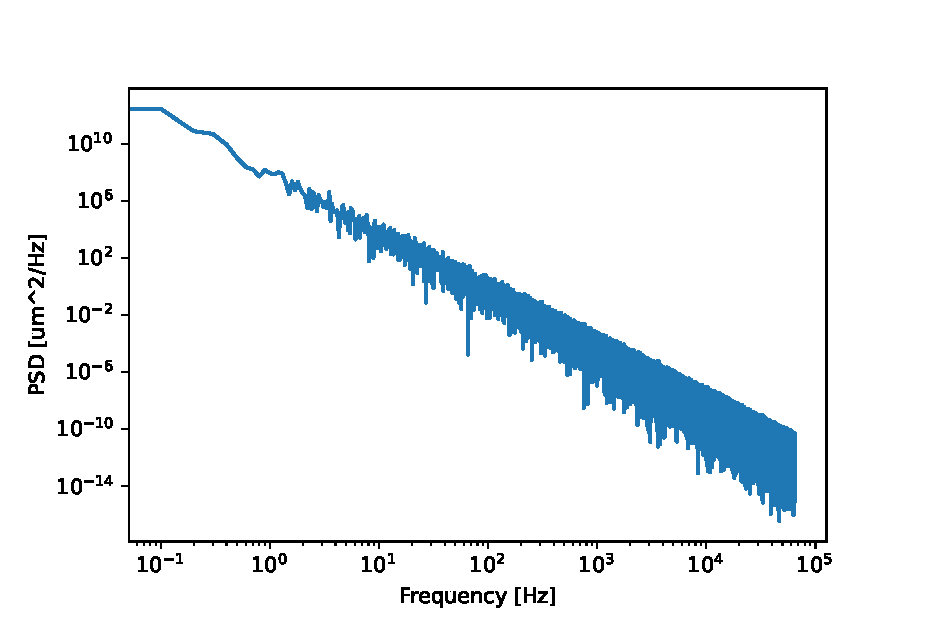
\includegraphics{power_spectrum.eps}
    \end{center}
    \caption{Simulated power spectrum at a single point.}
    \label{fig:power_spectrum}
\end{figure}

\subsection{Theorical Background}

\subsection{Simulation Model}

\subsection{Simulation Results}

\subsection{Robust Stability Analysis}

\subsection{pyAT}
}		%
	{\section {Schreiben am Institut für Regelungstechnik}
\label{a:ab_rts_en}


\subsection{Hardware-Ausstattung}

Im Rechnerraum N1.059 stehen PCs für Studenten zur Verfügung, die
generell sowohl für Berechnungen (meist mit \textsc{Matlab}/\textsc{Simulink}) als
auch für die Ausarbeitung des schriftlichen Teils genutzt werden
können.


\subsection{Verfügbare Software}

Als geeignete \LaTeX-Editoren haben sich
\begin{itemize}
    \item TeXnicCenter
    \item Texmaker
    \item TeXStudio
    \item Visual Studio Code + LatexWorkshop
\end{itemize}

bewährt.
Prinzipiell kann jeder Editor (z.B. LED) genutzt werden.
Damit haben Sie die richtigen Einstellungen zum Kompilieren und es sollte eine pdf-datei mit ihrer Arbeit erzeugt werden.
Ist dies nicht der Fall, überprüfen Sie Ihre Einstellungen, ob die Pfade zu den Programmen zur Nachbereitung und des Viewers stimmen. 

\subsection{Zitate aus der Literatur-Datenbank}

Das Institut verfügt über eine gemeinsame
Literatur-Datenbank, in der eine Vielzahl der Bücher und Artikel,
die Sie zitieren wollen, wahrscheinlich bereits enthalten sind. 
Das entsprechende bib-file, welches Sie mit Ihrem \LaTeX-Editor oder einem
Literaturverwaltungstool wie beispielsweise ''jabref'' öffnen können, 
finden Sie unter \verb"S:\ICS Library\ics.bib". 
Fragen Sie Ihren Betreuer/Betreuerin nach der aktuellsten Version und kopieren Sie diese in das Hauptverzeichnis Ihrer Arbeit.

Prüfen Sie, ob Ihre Literaturstelle enthalten ist. 
Dann können Sie einfache das \LaTeX-Kürzel in
den entsprechenden Befehl einfügen. Durch den Verweis auf die
Bib\TeX-Datei wird dann das
Literaturverzeichnis automatisch erstellt. Hierfür müssen Sie \texttt{biber} aufrufen.

Sollte das von Ihnen gewünschte Zitat noch nicht in der
Literaturdatenbank aufgeführt sein, sprechen Sie bitte mit Ihrem
Betreuer. Wir sind bemüht, die Datenbank um für uns wichtige
Dokumente zu erweitern und die Tatsache, dass die Literaturstelle
von Ihnen ausgewählt wurde, spricht schon für die Wichtigkeit! Wir
werden das dann in der Regel übernehmen und somit können Sie auch
''Ihr'' Zitat dann in der Datenbank finden. Es empfiehlt sich, die
Literaturliste bereits bei Beginn der Niederschrift mit dem Stand
der Datenbank zu vergleichen, damit zusätzliche Einträge oder
Änderungen nicht in letzter Minute noch eingepflegt werden müssen.
Es ist immer Hilfreich dem Betreuer vollständige Angaben zur Literaturstelle
zu machen: Titel, Autoren, Datum, DOI, vielleicht sogar ein PDF!


\subsection{Binden der Arbeit}

Am Arbeitsbereich gibt es die Möglichkeit, die fertige Arbeit zu drucken und zu
binden. Dazu fertigt man in der Regel drei Exemplare an (für den
Betreuer, den Professor und sich selbst), ggf.\ aber auch mehr.
Nachdem der Titel der Arbeit endgültig festgelegt ist, wird dieser
von Ihrem Betreuer in die Literaturdatenbank des Arbeitsbereiches
eingetragen. 

Ihre Arbeit wird in der korrekten Reihenfolge gedruckt. Vorne kommt eine Klarsichtfolie davor und dahinter eine Kartonseite.

Im Gegensatz zu einer Leimbindung, die auf den ersten Blick sehr
elegant aussieht, hat die Klammerbindung den unschätzbaren
Vorteil, dass sie auch nach Jahren nicht auseinander fällt. Suchen
Sie sich die Klammern in der richtigen Größe aus dem Regal im Computerpool und nutzen Sie die großen
Heftklammerapparate. Danach sollten Sie den Rücken der Arbeit noch
mit Gewebeband umkleben, unter dem die Klammern dann verschwinden.
Sie finden sicherlich Anschauungsmaterial in Form alter Arbeiten
in der Bibliothek.

Zur Abgabe ist auch eine CD/DVD, mit Ihrer Arbeit als pdf und allen wichtigen Dateien, nötig. Bitte ordnen Sie diese übersichtlich, damit auch Jahre später noch jemand daraus schlau werden kann. Die CD/DVD wird mit einer Papierhülle hinten in Ihre Arbeit geklebt.

Zu guter Letzt, denken Sie daran die Eigenständig\-keits\-erklärung zu unterschreiben, bevor Sie die Arbeit abgeben.} 	        %
	%
	\ifthenelse{\equal{\isenglish}{true}}%
	{\section{Conclusion and Outlook}

To complete}		        % Conclusion
	{\section {Zusammenfassung und Ausblick}

Der vorliegenden Text gibt Studentinnen und Studenten, die am
Beginn der Niederschrift Ihrer Bachelor- oder Masterarbeit am
Arbeitsbereich Regelungstechnik sind eine Anleitung, welche Punkte
zu beachten sind, damit diese Arbeit gelingt.


Sicherlich wurden nicht alle Aspekte des Schreibens aufgeführt.
Für weitere Fragen steht Ihnen ja Ihr Betreuer ebenso zu
Verfügung. Nutzen Sie den Dialog nach der Korrektur einzelner
Abschnitte als geeignetes Mittel zur Verbesserung Ihres
schriftlichen Textes!
} 	        % Zusammenfassung
	
	\printbibliography[title=\bibnamem]
\end{refsection} 

 %% Appendix ---------------------------------------------
\appendix

\end{document}
